\chapter{Hardware Anatomy}

\section{The Dual-Brain Architecture}
The system is divided into two distinct processing domains:
\begin{enumerate}
    \item \textbf{The Cortex (Raspberry Pi 4B)}: Handles High-Level logic, AI (Vision/Audio), and Networking.
    \item \textbf{The Brainstem (ESP32)}: Handles Low-Level reflexes, PWM signal generation, and Analog sensor reading.
\end{enumerate}

\begin{figure}[h]
    \centering
    % Placeholder for Block Diagram
    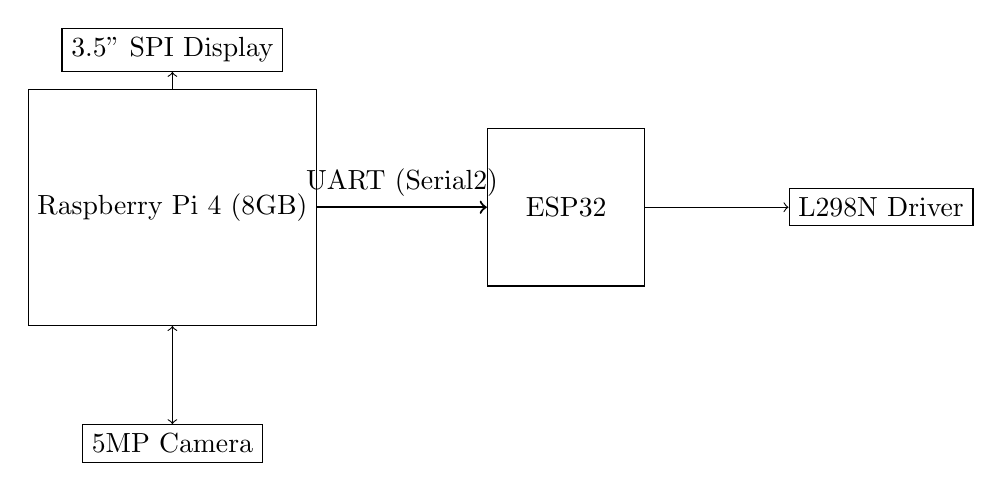
\begin{tikzpicture}
        \node[draw, minimum size=3cm] (pi) {Raspberry Pi 4 (8GB)};
        \node[draw, minimum size=2cm, right of=pi, node distance=5cm] (esp) {ESP32};
        \node[draw, below of=pi, node distance=3cm] (cam) {5MP Camera};
        \node[draw, above of=pi, node distance=2cm] (disp) {3.5" SPI Display};
        \node[draw, right of=esp, node distance=4cm] (motor) {L298N Driver};
        
        \draw[->, thick] (pi) -- node[above] {UART (Serial2)} (esp);
        \draw[<->] (pi) -- (cam);
        \draw[->] (pi) -- (disp);
        \draw[->] (esp) -- (motor);
    \end{tikzpicture}
    \caption{High-Level Hardware Wiring}
\end{figure}

\section{Power Distribution System}
Stable power is critical. We use two isolated rails sharing a \textbf{Common Ground}.
\begin{itemize}
    \item \textbf{Rail A (Logic)}: Official Raspberry Pi USB-C Supply (5.1V, 3A). Powers the Pi, Camera, USB Mic, and Display.
    \item \textbf{Rail B (Drive)}: Li-Ion Battery Pack. Powers the L298N Motor Driver and ESP32.
\end{itemize}
\textbf{Critical Engineering Detail}: The Common Ground ensures that UART logic levels (3.3V) between the Pi and ESP32 are referenced to the same 0V potential, preventing communication errors.

\section{Motor Drive Subsystem}
\begin{itemize}
    \item \textbf{Driver}: L298N H-Bridge.
    \item \textbf{Motors}: 4x DC Gear Motors.
    \item \textbf{Control Logic}: The Pi sends a command (e.g., `FORWARD`). The ESP32 asserts HIGH on relevant pins.
    \item \textbf{Pinout (ESP32)}:
    \begin{itemize}
        \item IN1 (Left Fwd): Pin 25
        \item IN2 (Left Bwd): Pin 26
        \item IN3 (Right Fwd): Pin 27
        \item IN4 (Right Bwd): Pin 14
    \end{itemize}
\end{itemize}

\section{Sensory Array}
\subsection{Ultrasonic (Sonar)}
Three HC-SR04 sensors provide a 180-degree collision map.
\begin{itemize}
    \item \textbf{Left (S1)}: Trig 4 / Echo 5
    \item \textbf{Center (S2)}: Trig 18 / Echo 19
    \item \textbf{Right (S3)}: Trig 21 / Echo 22
\end{itemize}

\subsection{Olfactory (Gas)}
An **MQ3 Alcohol/Gas Sensor** is connected to the ESP32's ADC.
\begin{itemize}
    \item \textbf{Pin}: GPIO 34 (Input only, ADC1\_6).
    \item \textbf{Usage}: Detects hazardous environments. Data is streamed as a raw 12-bit integer (0-4095).
\end{itemize}

\subsection{Visual Status (Neopixel)}
An 8-LED Adafruit Ring is connected to the Pi (GPIO 12).
\begin{itemize}
    \item \textbf{Role}: Shows system state (Blue=Listening, Green=Moving, Red=Error).
    \item \textbf{Power}: 5V from Pi GPIO header (consumes ~400mA at full white, safe for Pi 4).
\end{itemize}
